\documentclass[dvips,12pt]{article}

\usepackage[pdftex]{graphicx}
\usepackage{subcaption}
\usepackage{float}
\usepackage{url}
\usepackage[utf8]{inputenc}
\usepackage{geometry}
\usepackage{setspace}
\usepackage{amsmath}
\usepackage{txfonts}

% From amsmath, prepend equation numbers with section number
%\numberwithin{equation}{section}

% graphicx: Where should graphics be found?
\graphicspath{ {figures/} }

% Setup margins and paper size
\geometry{
  letterpaper,
  total={170mm,257mm},
  left=20mm,
  top=20mm,
  bottom=25mm
}

\setcounter{MaxMatrixCols}{20}

\makeatletter % changes the catcode of @ to 11
\renewcommand*\env@matrix[1][*\c@MaxMatrixCols c]{%
  \hskip -\arraycolsep
  \let\@ifnextchar\new@ifnextchar
  \array{#1}}
\makeatother % changes the catcode of @ back to 12

% -----------------------------------------------------------------------------

\begin{document}

% Article Title
\title{\LARGE The Desktop Quad \\ \large with an LQR setpoint controller }
\author{Parker Lusk}
\date{\today}
\maketitle

\begin{abstract}
	The Desktop Quad is an effort to allow an inexpensive quadrotor to be used as a case study in controls, vision processing, and autopilot design scenarios. It features an 8cm x 8cm quadrotor with an upward-facing camera for localization. The (really) micro air vehicle (MAV) is tethered using silicone wire for communications and power, allowing indefinite flight. This report describes the progress of the Desktop Quad achieving fully autonomous flight.
\end{abstract}

\doublespacing
% -----------------------------------------------------------------------------
\section{Introduction}
My project was to add an LQR setpoint controller to a multirotor system.

% -----------------------------------------------------------------------------
\section{System Modeling}
We begin by modeling the Desktop Quad multirotor and deriving the equations of motion. The 12 state variables that will be used to describe the equations of motions are

\begin{equation*}
x =
\begin{bmatrix}
p_n & p_e & p_d & \dot{p_n} & \dot{p_e} & \dot{p_d} & \phi & \theta & \psi & p & q & r
\end{bmatrix}
^T
\end{equation*}

\noindent where all the states are inertial coordinate frame quantities except for the angular rates $p$, $q$, and $r$ which are in the body frame.

\subsection{Kinematics and Dynamics}
In order to analyze, simulate, and control the Desktop Quad, a 6DOF dynamic model must be derived. This is done using kinematics and dynamics. The goal is to find the evolution equations for each of the quantities we care about, as found in the state vector above.

\singlespacing
\begin{equation}
\begin{bmatrix}
\ddot{p_n} \\
\ddot{p_e} \\
\ddot{p_d} \\
\end{bmatrix}
=
R_b^i(\phi, \theta, \psi)
\begin{bmatrix}
0  \\
0  \\
-T \\
\end{bmatrix}
\frac{1}{m} +
\begin{bmatrix}
0 \\
0 \\
g \\
\end{bmatrix}
\end{equation}
\doublespacing

\singlespacing
\begin{equation}
\begin{bmatrix}
\dot{\phi} \\
\dot{\theta} \\
\dot{\psi} \\
\end{bmatrix}
=
\begin{bmatrix}
1 & s_{\psi}t_{\theta} & c_{\phi}t_{\theta} \\
0 & c_{\phi}           & -s_{\phi}          \\
0 & \frac{s_{\phi}}{c_{\theta}} & \frac{c_{\phi}}{c_{\theta}} \\
\end{bmatrix}
\begin{bmatrix}
p \\
q \\
r \\
\end{bmatrix}
\end{equation}
\doublespacing

\singlespacing
\begin{equation}
\begin{bmatrix}
\dot{p} \\
\dot{q} \\
\dot{r} \\
\end{bmatrix}
=
\begin{bmatrix}
\Gamma_1pq - \Gamma_2qr \\
\Gamma_5pr - \Gamma_6(p^2-r^2) \\
\Gamma_7pq - \Gamma_1qr \\
\end{bmatrix}
+
\begin{bmatrix}
\Gamma_3l + \Gamma_4n \\
\frac{1}{J_y}m \\
\Gamma_4l + \Gamma_8n \\
\end{bmatrix}
\end{equation}
\doublespacing

\subsection{Forces and Moments}

% -----------------------------------------------------------------------------
\section{Control Architecture}

The Desktop Quad uses the ROSflight \cite{rosflight} stack for autonomous flight and thus has an on-board autopilot for attitude control. This simplifies the control problem and eliminates the need to control the moments $l$, $m$, and $n$. The LQR controller developed here will close the attitude loop using a position setpoint controller with the simplified state vector

\singlespacing
\begin{equation*}
x =
\begin{bmatrix}
p_n & p_e & p_d & \dot{p_n} & \dot{p_e} & \dot{p_d} & \psi
\end{bmatrix}
^T
\end{equation*}
\doublespacing

\noindent with input to the ROSflight autopilot

\singlespacing
\begin{equation*}
\nu =
\begin{bmatrix}
T & \phi & \theta & r
\end{bmatrix}^T.
\end{equation*}
\doublespacing

Because of how we have defined our state, we will need to create a nonlinear map between the control $u$ produced by our controller and the input $\nu$ to the autopilot. We can use the kinematic and dynamic relationships to define the map

\begin{equation}
\boldsymbol{u} = 
\begin{bmatrix}
u_{p_{3x1}} \\
u_{{\psi}_{1x1}}
\end{bmatrix},
\end{equation}

\noindent where

\begin{equation}
u_p =
R_b^i(\phi, \theta, \psi)
\begin{bmatrix}
0  \\
0  \\
-T \\
\end{bmatrix}
\frac{1}{m}
\end{equation}

\noindent and

\begin{equation}
u_{\psi} =
q\frac{sin\phi}{cos\theta} + r\frac{cos\phi}{cos\theta}.
\end{equation}

\noindent Inverting these relationships will give us a mapping for how $u$ affects $\nu$, which can be feed into autopilot. The state-space system can be represented as

\begin{equation}
\dot{x} = Ax + Bu + bg
\end{equation}

\noindent with


\begin{equation}
A =
\begin{bmatrix}
0_{3x3} & I_{3x3} & 0_{3x1} \\
0_{3x3} & 0_{3x3} & 0_{3x1} \\
0_{1x3} & 0_{1x3} & 0_{1x1} \\
\end{bmatrix}
, \quad
B =
\begin{bmatrix}
0_{3x3} & 0_{3x1} \\
I_{3x3} & 0_{3x1} \\
0_{1x3} & 1 \\
\end{bmatrix}
, \quad
b = [0 \enspace 0 \enspace 0 \enspace 0 \enspace 0 \enspace 1 \enspace 0]^T
\end{equation}


% -----------------------------------------------------------------------------
\section{Building the System}

% -----------------------------------------------------------------------------
\section{Visual Localization}

% -----------------------------------------------------------------------------
\section{Simulation}

% -----------------------------------------------------------------------------
\section{Control Architecture}

\begin{figure}[H]
	\centering
	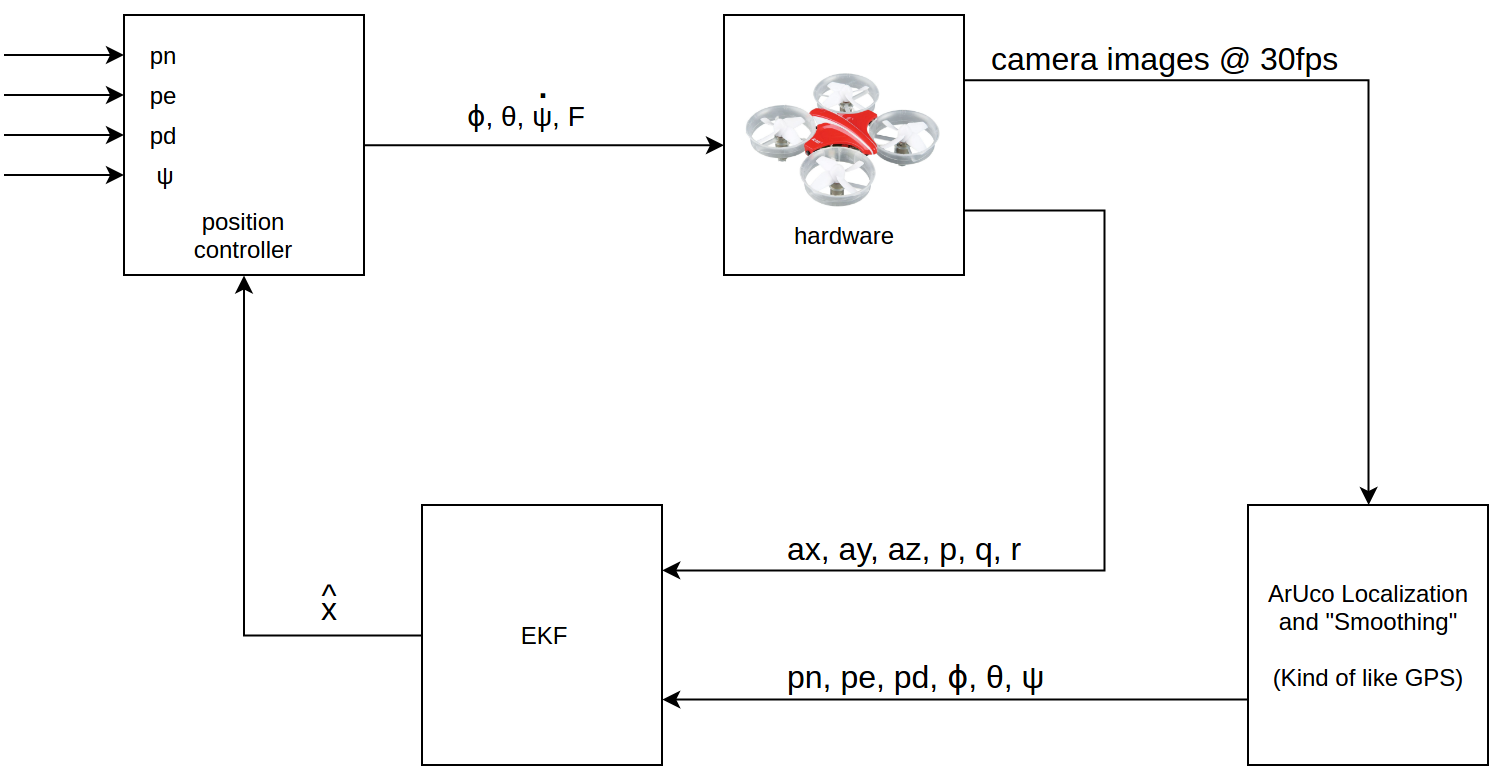
\includegraphics[width=\textwidth]{desktopquad_control_arch}
	\caption{Control architecture of the Desktop Quad system.}
	\label{fig:architecture}
\end{figure}


\begin{thebibliography}{9}
\singlespace

\bibitem{UAVBook} R. W. Beard and T. W. McLain, “Small unmanned aircraft,” 2011.

\bibitem{Beard2016} R. W. Beard and T. W. Mclain, “Introduction to Feedback Control using Design Studies,” 2016.

\bibitem{Ferrin2011} J. Ferrin, R. Leishman, R. Beard, and T. McLain, “Differential flatness based control of a rotorcraft for aggressive maneuvers,” IEEE Int. Conf. Intell. Robot. Syst., pp. 2688–2693, 2011.

\bibitem{rosflight} J. Jackson, G. Ellingson, and T. McLain, “ROSflight: A lightweight, inexpensive MAV research and development tool,” 2016 Int. Conf. Unmanned Aircr. Syst. ICUAS 2016, pp. 758–762, 2016.

\bibitem{Albasiouny2016} E. R. Albasiouny, A. Sarhan, and T. Medhat, “Mean-shift-FAST algorithm to handle motion-blur with tracking fiducial markers,” Proc. - 2015 10th Int. Conf. Comput. Eng. Syst. ICCES 2015, no. December, pp. 286–292, 2016.

\bibitem{aruco2014} S. Garrido-Jurado, R. Muñoz-Salinas, F. J. Madrid-Cuevas, and M. J. Marín-Jiménez, “Automatic generation and detection of highly reliable fiducial markers under occlusion,” Pattern Recognit., vol. 47, no. 6, pp. 2280–2292, 2014.

\bibitem{apriltag2011} E. Olson, “AprilTag: A robust and flexible visual fiducial system,” Proc. - IEEE Int. Conf. Robot. Autom., pp. 3400–3407, 2011.

\bibitem{Prasad2015} M. G. Prasad, S. Chandran, and M. S. Brown, “A motion blur resilient fiducial for quadcopter imaging,” Proc. - 2015 IEEE Winter Conf. Appl. Comput. Vision, WACV 2015, pp. 254–261, 2015.

\end{thebibliography}

\end{document}